\documentclass[11pt,a4paper]{article}
\usepackage[T1]{fontenc}
\usepackage[utf8]{inputenc}
\usepackage[brazil]{babel}
\usepackage{lmodern}
\usepackage{microtype}
\usepackage{amsmath,amssymb,mathtools,amsthm}
\usepackage{geometry}
\usepackage{booktabs,tabularx,array}
\usepackage{graphicx}
\usepackage{hyperref}
\geometry{margin=2.4cm}
\hypersetup{colorlinks=true,linkcolor=black,citecolor=black,urlcolor=blue}
\newtheorem{theorem}{Teorema}[section]
\newtheorem{corollary}[theorem]{Corolário}
\setlength{\parindent}{1.2em}
\setlength{\parskip}{0.15em}

\title{\textbf{Geometria de Relaxações Contínuas de 3-SAT}\\[0.3em]
\large Platôs Hinge, paisagens multilineares harmônicas e convexidade Softplus}
\author{Thiago Carvalho\\Pesquisador independente\\\texttt{thiagocarvalho.dba@gmail.com}}
\date{Rascunho para análise -- derivado da fonte auditada CLG-R v4.0.5 (setembro de 2026)}

\begin{document}
\maketitle

\begin{abstract}
Comparamos três representações contínuas de 3-SAT no hipercubo $[-1,1]^N$: uma penalidade Hinge quadrática da relaxação linear cláusula a cláusula, a extensão multilinear natural da contagem Booleana de violações e uma suavização Softplus das mesmas violações afins de cláusula. Embora as três estejam ligadas à mesma estrutura discreta de cláusulas, suas geometrias interiores são qualitativamente distintas. Provamos que a relaxação Hinge contém a caixa fracionária central universal $(-1/3,1/3)^N$, na qual energia e gradiente se anulam, fornecendo uma manifestação geométrica direta da folga interior $0{,}5$ da relaxação linear por cláusula. Sob uma condição de não degenerescência do objetivo Booleano, os conjuntos críticos das relaxações multilinear e Softplus têm medida de Lebesgue zero. A extensão multilinear é harmônica, portanto não possui mínimos locais interiores; todo ponto crítico interior não degenerado é uma sela, e todo mínimo local estrito no cubo projetado é um vértice Booleano. Em contraste, a Hessiana Softplus se fatoriza globalmente como $V^TW(x)V\succeq0$ e torna-se definida positiva quando a matriz de incidência de cláusulas tem posto de coluna completo. Derivamos cotas espectrais e de Lipschitz explícitas, incluindo o escalonamento linear $L_\beta=\Theta(\beta)$ com a temperatura inversa de suavização. Finalmente, para o fluxo Hinge quadrático, provamos uma identidade universal de contração centrípeta e mostramos que o conjunto de equilíbrios projetados coincide exatamente com o politopo LP cláusula a cláusula. Esses resultados mostram que a geometria da representação, e não apenas os valores Booleanos nos vértices, é uma propriedade matematicamente decisiva das formulações contínuas de SAT.
\end{abstract}

\noindent\textbf{Palavras-chave.} 3-SAT; relaxação contínua; funções harmônicas; fluxo de gradiente projetado; Softplus; convexidade; relaxação LP.

\section{Configuração e três representações contínuas}
Seja $F$ uma fórmula 3-CNF com $M$ cláusulas sobre $N$ variáveis e seja $\sigma^{(c)}\in\{-1,0,+1\}^N$ o vetor de polaridades da cláusula $c$. Assumimos que cada cláusula contém exatamente três variáveis distintas e que toda variável aparece em ao menos uma cláusula. Defina
\begin{equation}
g_c(x)=-\frac12\bigl(1+\sigma^{(c)}\cdot x\bigr),\qquad x\in\mathcal X=[-1,1]^N.
\end{equation}
Em um vértice Booleano $s\in\{-1,+1\}^N$, $g_c(s)=1$ exatamente quando a cláusula $c$ é violada.

Estudamos três potenciais:
\begin{align}
\Phi_{\mathrm{quad}}(x)&=\sum_{c=1}^M[\max(0,g_c(x))]^2,\\
\Phi_{\mathrm{mult}}(x)&=\sum_{c=1}^M\prod_{j\in c}\frac{1-\sigma_j^{(c)}x_j}{2},\\
\Phi_{\mathrm{soft}}(x)&=\sum_{c=1}^M\frac1\beta\log\bigl(1+e^{\beta g_c(x)}\bigr),\qquad \beta>0.
\end{align}
A dinâmica é o fluxo de gradiente projetado
\begin{equation}
\dot x=\Pi_{T_{\mathcal X}(x)}(-\nabla\Phi(x)).
\end{equation}
Para as afirmações de medida zero das versões multilinear e Softplus, assumimos que a energia Booleana não é constante, equivalentemente $\operatorname{Var}(E_{\mathrm{disc}})>0$.

\section{O platô Hinge universal}
Defina
\[
\mathcal U_N=(-1/3,1/3)^N.
\]
\begin{theorem}[Caixa fracionária central]
Para toda fórmula 3-CNF,
\[
\Phi_{\mathrm{quad}}(x)=0,\qquad \nabla\Phi_{\mathrm{quad}}(x)=0,
\qquad \forall x\in\mathcal U_N.
\]
Logo o volume normalizado do politopo LP de energia zero é pelo menos $(1/3)^N$. Se a energia Booleana é não constante, pelo menos um ortante de sinais dentro de $\mathcal U_N$ arredonda para uma atribuição Booleana que viola alguma cláusula, e o conjunto crítico espúrio tem medida normalizada pelo menos $(1/6)^N$.
\end{theorem}
\begin{proof}
Para $x\in\mathcal U_N$ e qualquer cláusula,
\[
\sum_{j\in c}\sigma_j^{(c)}x_j>-3(1/3)=-1,
\]
logo $g_c(x)<0$. Todos os termos Hinge estão, portanto, simultaneamente inativos.
\end{proof}

Para uma cláusula fixa, introduza coordenadas de satisfação literal
\[
q_{cj}=\frac{1+\sigma_j^{(c)}x_j}{2}.
\]
Então $g_c(x)\le0$ é equivalente a $\sum_{j\in c}q_{cj}\ge1$. Na origem, todo $q_{cj}=1/2$, de modo que a desigualdade LP possui folga exata $3/2-1=0{,}5$. O platô não é um acidente numérico: é o interior geométrico da relaxação linear por cláusula.

\begin{figure}[htbp]
\centering
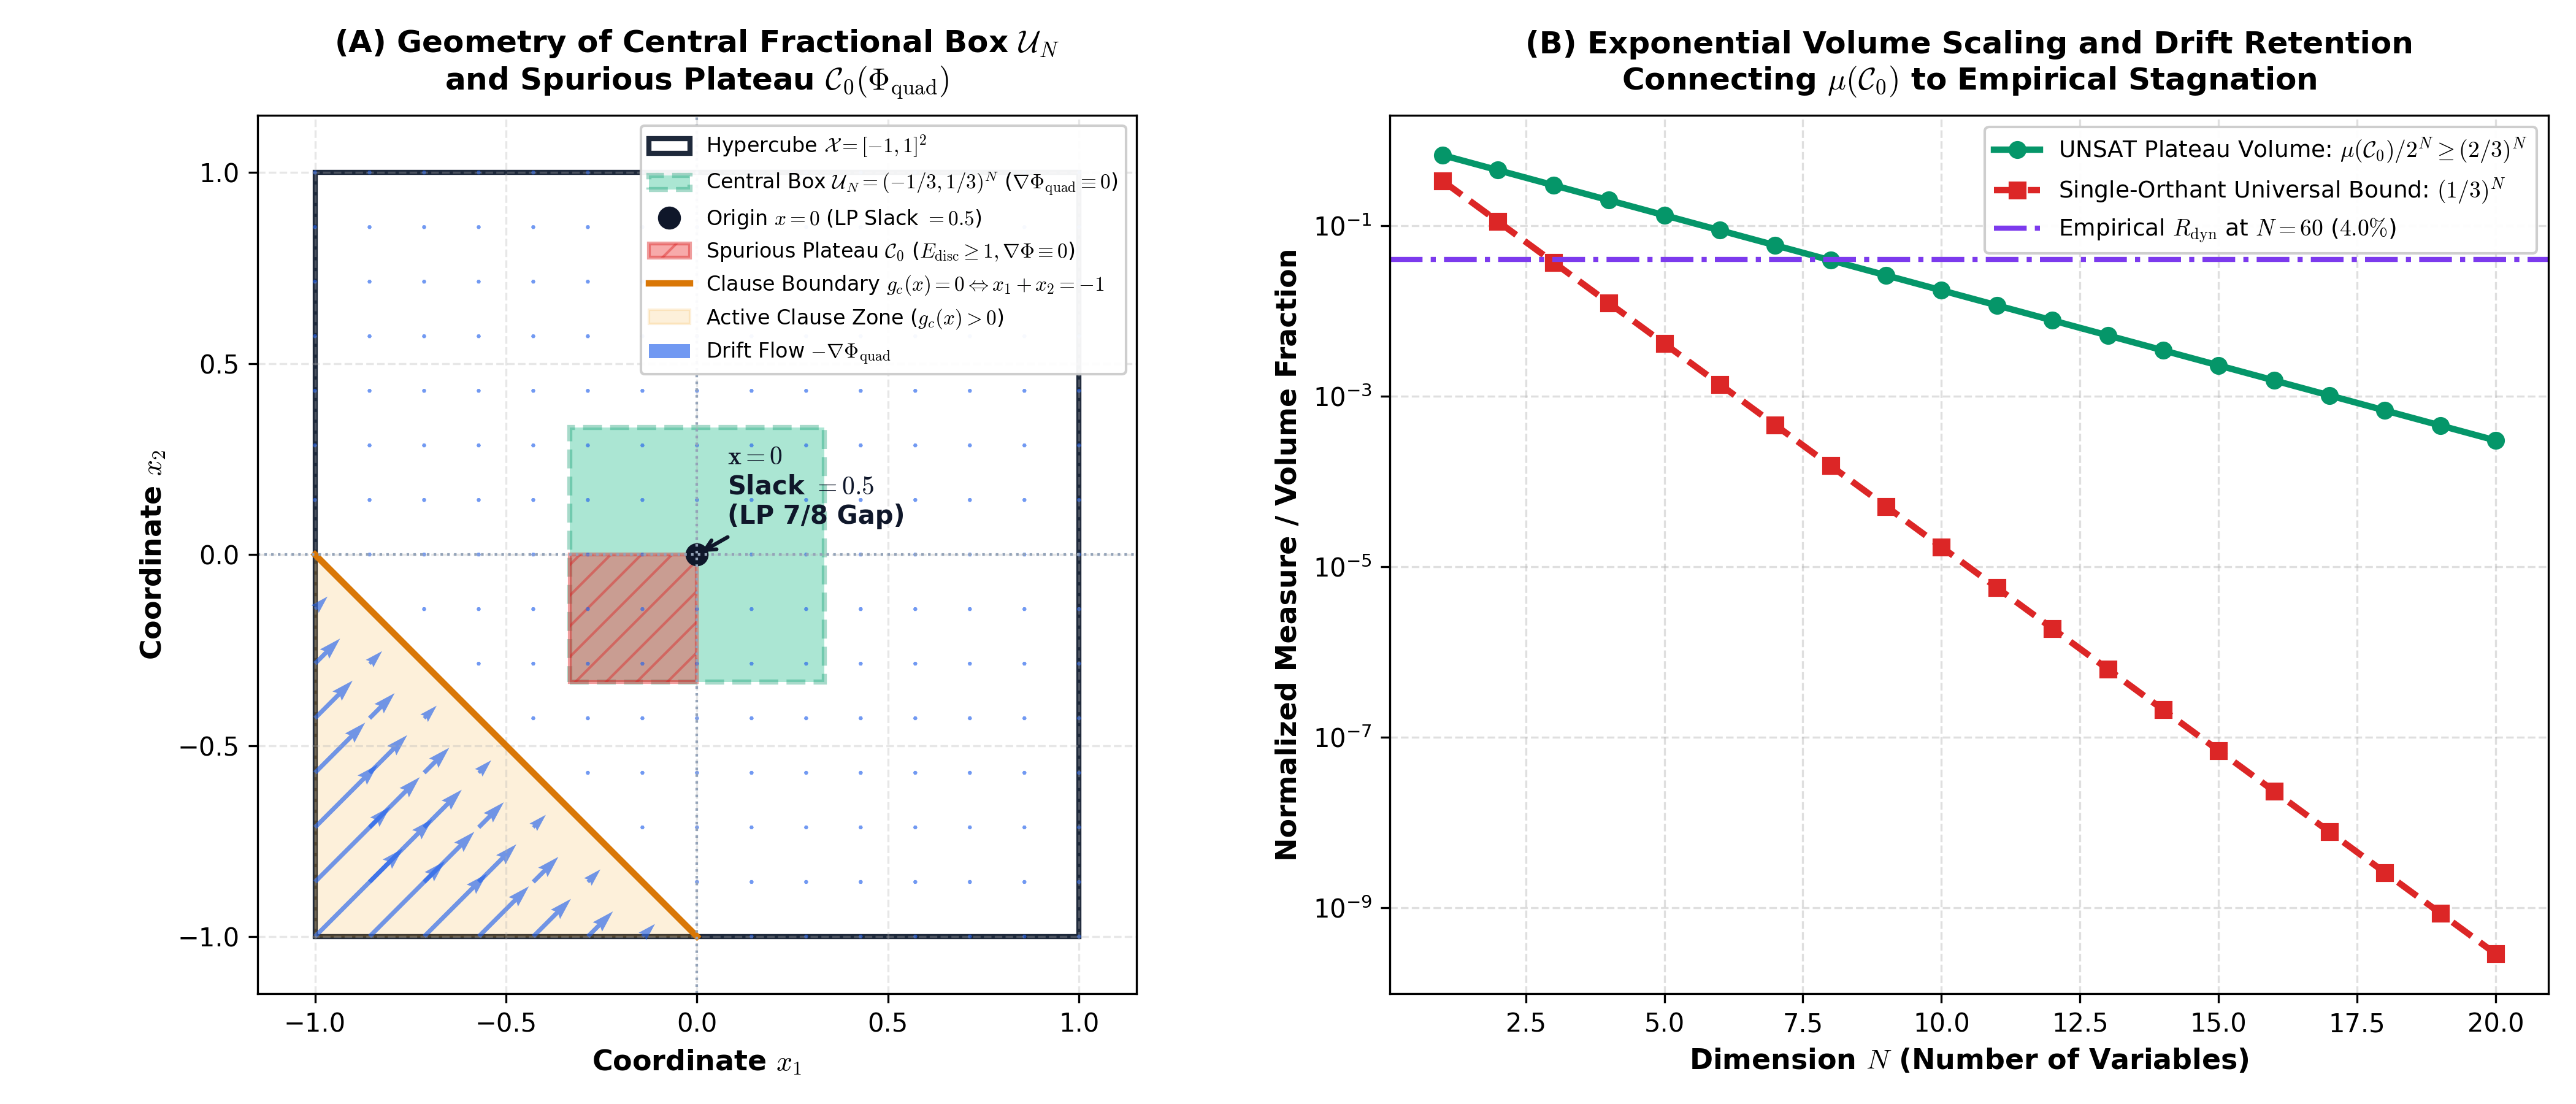
\includegraphics[width=0.80\textwidth]{../../fig_clg_teorema1_caixa_fracionaria.png}
\caption{Ilustração da caixa fracionária central e de sua escala de volume exponencial. O resultado usado aqui é a inclusão determinística $\mathcal U_N\subseteq Z$.}
\end{figure}

\section{Conjuntos críticos de medida zero fora do platô Hinge}
\begin{theorem}[Conjuntos críticos analíticos]
Se a energia Booleana é não constante, então
\[
\mu\{\nabla\Phi_{\mathrm{mult}}=0\}=0,
\qquad
\mu\{\nabla\Phi_{\mathrm{soft}}=0\}=0.
\]
\end{theorem}
\begin{proof}
O potencial multilinear é um polinômio não constante. Portanto, ao menos uma derivada parcial é um polinômio não nulo, cujo conjunto de zeros tem medida de Lebesgue zero \cite{okamoto1973distinctness,caron2005zero}; o conjunto crítico completo está contido nesse zero-set.

O potencial Softplus é real-analítico. Sua fatoração Hessiana abaixo implica
\[
\Delta\Phi_{\mathrm{soft}}(x)=\frac34\sum_{c=1}^M w_c(x)>0,
\]
logo ele não é constante. Ao menos uma derivada parcial é então uma função real-analítica não trivial, e seu conjunto de zeros tem medida zero \cite{krantz2002primer}.
\end{proof}

\section{Harmonicidade da extensão multilinear}
\begin{theorem}[Estrutura harmônica de selas]
O potencial multilinear satisfaz
\[
\Delta\Phi_{\mathrm{mult}}\equiv0.
\]
Consequentemente, não há mínimo local interior. Todo ponto crítico interior não degenerado é uma sela hiperbólica com ao menos um autovalor Hessiano positivo e um negativo, e todo ponto crítico interior possui pontos de energia inferior em qualquer vizinhança.
\end{theorem}
\begin{proof}
Cada termo de cláusula é multilinear em variáveis distintas, logo toda derivada segunda pura $\partial_{ii}^2\Phi_{\mathrm{mult}}$ se anula. O Princípio do Mínimo Forte exclui mínimos locais interiores de uma função harmônica não constante \cite{courant1962methods,evans2010partial}. Em um ponto crítico não degenerado, a Hessiana simétrica é inversível e tem traço zero, forçando autovalores de ambos os sinais. O caso degenerado segue diretamente da ausência de mínimo local; um argumento de seleção de curvas pode reforçar a conclusão para um arco analítico descendente \cite{milnor1968singular}.
\end{proof}

\begin{figure}[htbp]
\centering
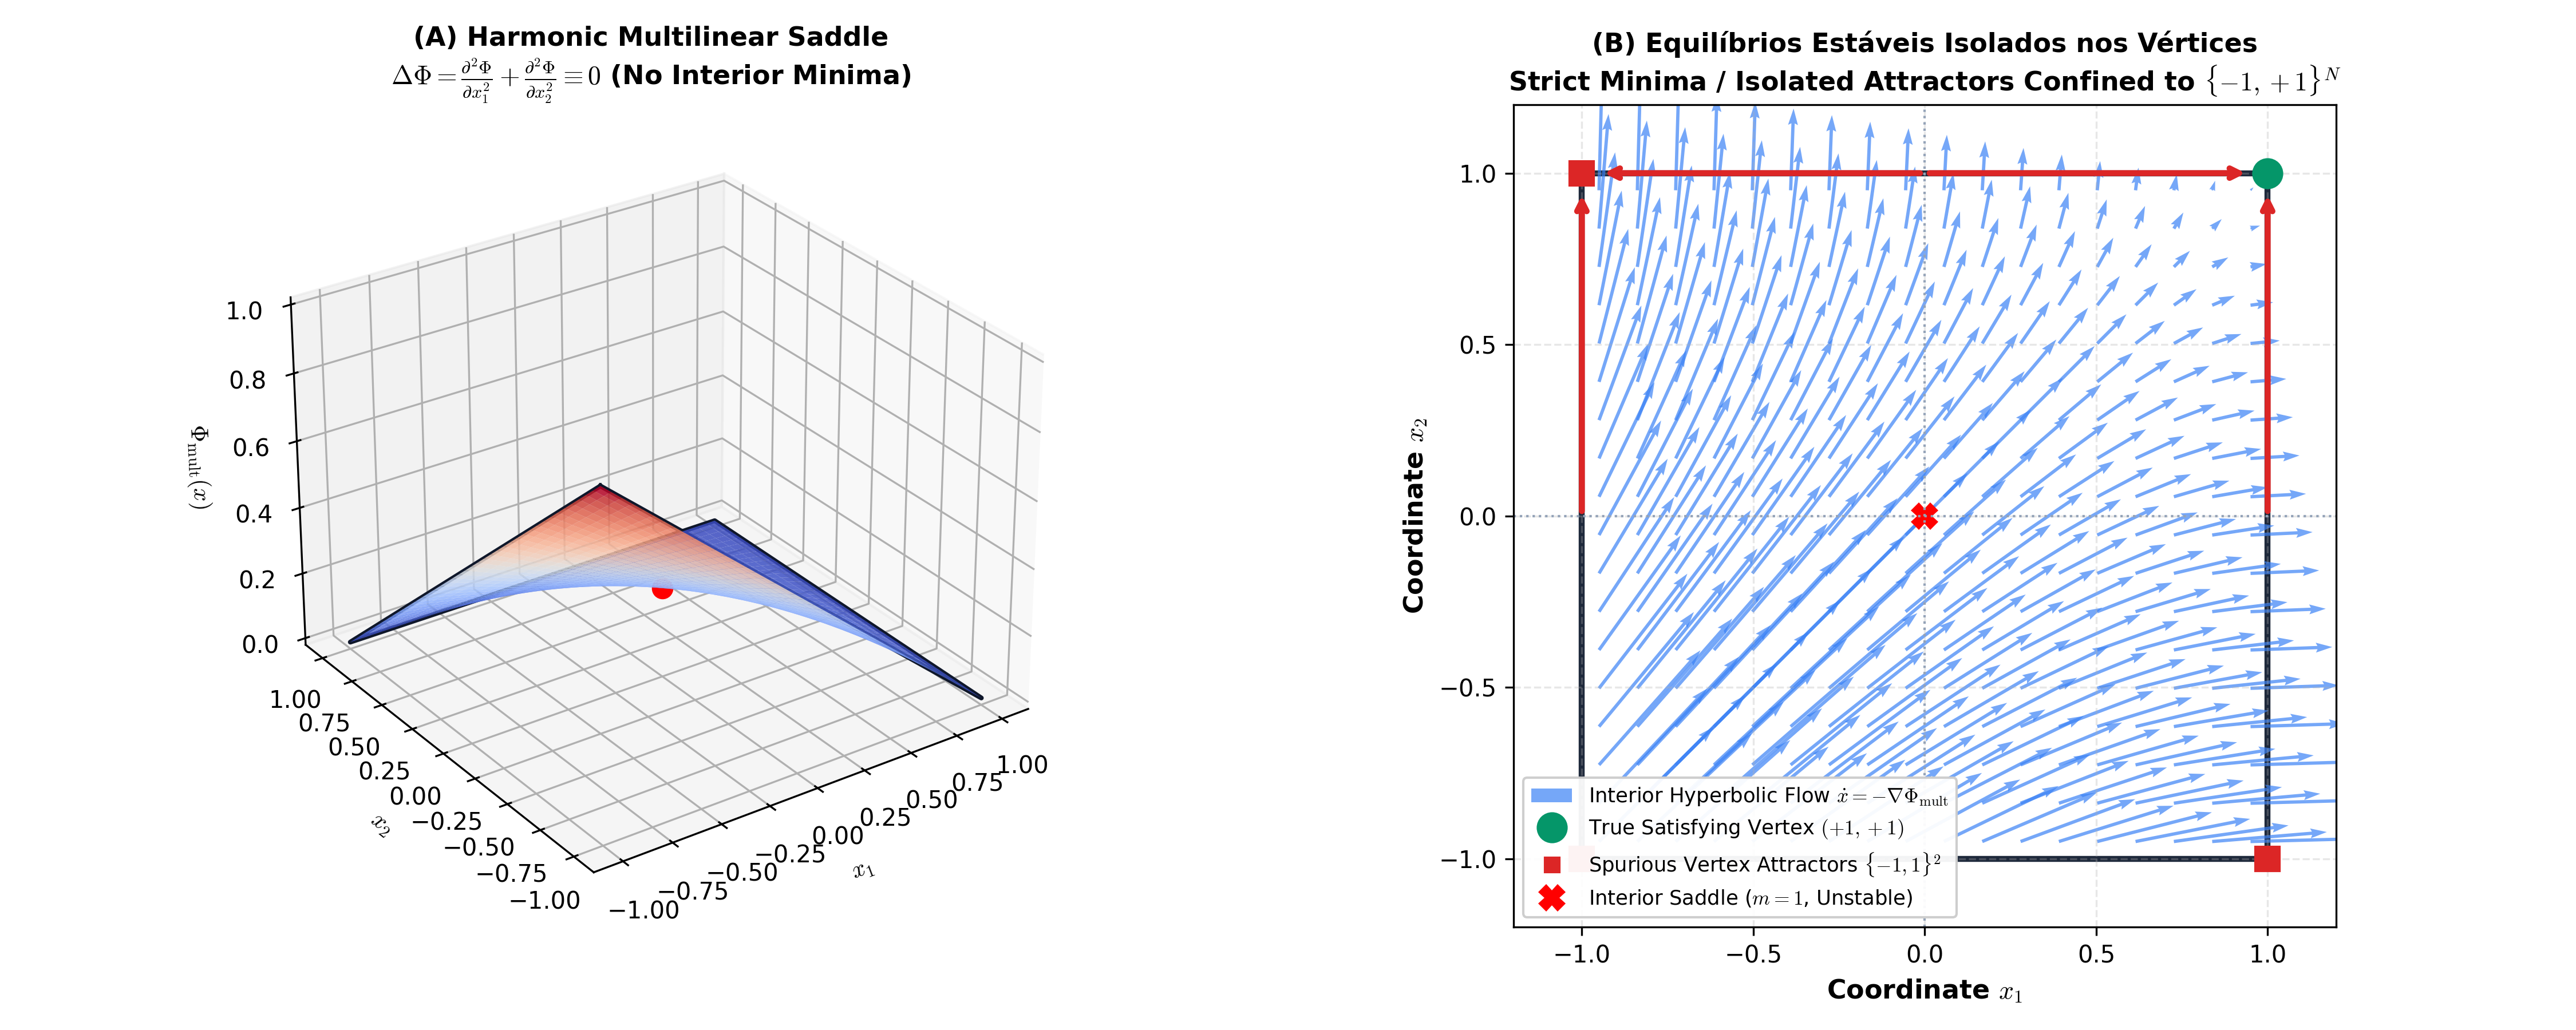
\includegraphics[width=0.80\textwidth]{../../fig_clg_teorema3_4_harmonic_saddles_vertices.png}
\caption{Geometria harmônica de selas e confinamento de equilíbrios projetados isolados e estáveis aos vértices Booleanos.}
\end{figure}

\section{Faces de bordo e atratores projetados}
O cubo é estratificado pelas interiores relativos de suas faces. Fixar coordenadas em $\pm1$ preserva a multilinearidade nas coordenadas restantes, de modo que o Laplaciano intrínseco em toda face de dimensão positiva também se anula.

\begin{theorem}[Mínimos em faces herdam a energia dos vértices]
Seja $x^*$ um mínimo local relativo de $\Phi_{\mathrm{mult}}$ no interior relativo de uma face $\mathcal F$. Então $\Phi_{\mathrm{mult}}$ é constante em $\mathcal F$ e
\[
\Phi_{\mathrm{mult}}(x^*)=E_{\mathrm{disc}}(v)
\quad\text{para todo vértice Booleano }v\in\mathcal V(\mathcal F).
\]
Em particular, todo mínimo local estrito relativo ao cubo inteiro é um vértice Booleano.
\end{theorem}

\begin{corollary}[Equilíbrios estáveis isolados são vértices]
Sob fluxo de gradiente multilinear projetado, todo equilíbrio assintoticamente estável e isolado pertence a $\{-1,+1\}^N$.
\end{corollary}
\begin{proof}
A projeção de Moreau fornece
\[
\frac{d}{dt}\Phi_{\mathrm{mult}}(x(t))
=-\|\Pi_{T_{\mathcal X}(x)}(-\nabla\Phi_{\mathrm{mult}})\|^2\le0.
\]
Um equilíbrio assintoticamente estável e isolado deve ser um mínimo local estrito: estados próximos de energia inferior não podem convergir "para cima", enquanto um ponto distinto de mesma energia ou decresce imediatamente abaixo da energia do equilíbrio ou já é outro equilíbrio. O teorema anterior força então uma face de dimensão zero.
\end{proof}

A palavra \emph{isolado} é essencial. Contínuos atratores não estritos e de dimensão positiva podem existir em faces de bordo; a construção M6 de seis cláusulas fornece um exemplo explícito em análise separada.

\section{Fatoração Hessiana e condicionamento do Softplus}
Seja $V\in\mathbb R^{M\times N}$ com linha $v_c^T=-\frac12(\sigma^{(c)})^T$. Defina
\[
w_c(x)=\beta\,\sigma(\beta g_c(x))\bigl(1-\sigma(\beta g_c(x))\bigr)>0,
\qquad W(x)=\operatorname{diag}(w_1,\ldots,w_M),
\]
onde $\sigma(u)=(1+e^{-u})^{-1}$ é a função logística.

\begin{theorem}[Fatoração Hessiana exata]
\[
\nabla^2\Phi_{\mathrm{soft}}(x)=V^TW(x)V\succeq0.
\]
Assim, $\Phi_{\mathrm{soft}}$ é globalmente convexa. Se $\operatorname{rank}(V)=N$, é estritamente convexa e
\[
\kappa(\nabla^2\Phi_{\mathrm{soft}})
\le \kappa(W)\,\kappa(V^TV).
\]
\end{theorem}
\begin{proof}
Como $g_c(x)=v_c^Tx-1/2$,
\[
\nabla\Phi_{\mathrm{soft}}=V^T\sigma(\beta g),
\qquad
\nabla^2\Phi_{\mathrm{soft}}=V^TWV.
\]
Para todo $z$, $z^TV^TWVz=\|W^{1/2}Vz\|^2\ge0$. As cotas de Courant--Fischer fornecem a estimativa do número de condição quando $V^TV$ é definida positiva.
\end{proof}

\section{Rigidez do Softplus e precisão finita}
Seja $d_{\max}$ o número máximo de cláusulas incidentes a uma variável.

\begin{theorem}[Escala Lipschitz do gradiente]
Defina a constante Lipschitz global por
\[
L_\beta=\sup_x\|\nabla^2\Phi_{\mathrm{soft}}(x)\|_2.
\]
Então
\[
\frac3{16}\beta\le L_\beta\le\frac{3d_{\max}}{16}\beta.
\]
Para $\mathcal U_N(\rho)=(-\rho,\rho)^N$, com $\rho<1/3$,
\[
\|\nabla\Phi_{\mathrm{soft}}\|_\infty
\le\frac M2e^{-\beta(1-3\rho)/2},
\qquad
\|\nabla\Phi_{\mathrm{soft}}\|_2
\le\frac{\sqrt3M}{2}e^{-\beta(1-3\rho)/2}.
\]
\end{theorem}
\begin{proof}
Como $w_c\le\beta/4$,
\[
\|\nabla^2\Phi_{\mathrm{soft}}\|_2\le\frac\beta4\lambda_{\max}(V^TV).
\]
A soma absoluta da linha de $V^TV$ associada à variável $i$ é no máximo $3d_i/4$; Gershgorin fornece a cota superior. Se $g_c(x)=0$ para uma cláusula, então $w_c=\beta/4$ e o termo de posto um possui valor espectral $(\beta/4)\|v_c\|^2=3\beta/16$, fornecendo a cota inferior. As estimativas no box central seguem de $g_c\le-(1-3\rho)/2$ e $\sigma(u)\le e^u$ para $u\le0$.
\end{proof}

Na origem, a escala exponencial relevante é $e^{-\beta/2}$. A fonte auditada distingue, em binary32, os cruzamentos ideais do menor normal, menor subnormal e meia unidade subnormal de arredondamento a zero aproximadamente em $174{,}67$, $206{,}56$ e $207{,}94$; os valores correspondentes para binary64 são $1416{,}79$, $1488{,}88$ e $1490{,}27$. São escalas do fator exponencial, e não limiares universais para uma implementação concreta de sigmoid.

\begin{figure}[htbp]
\centering
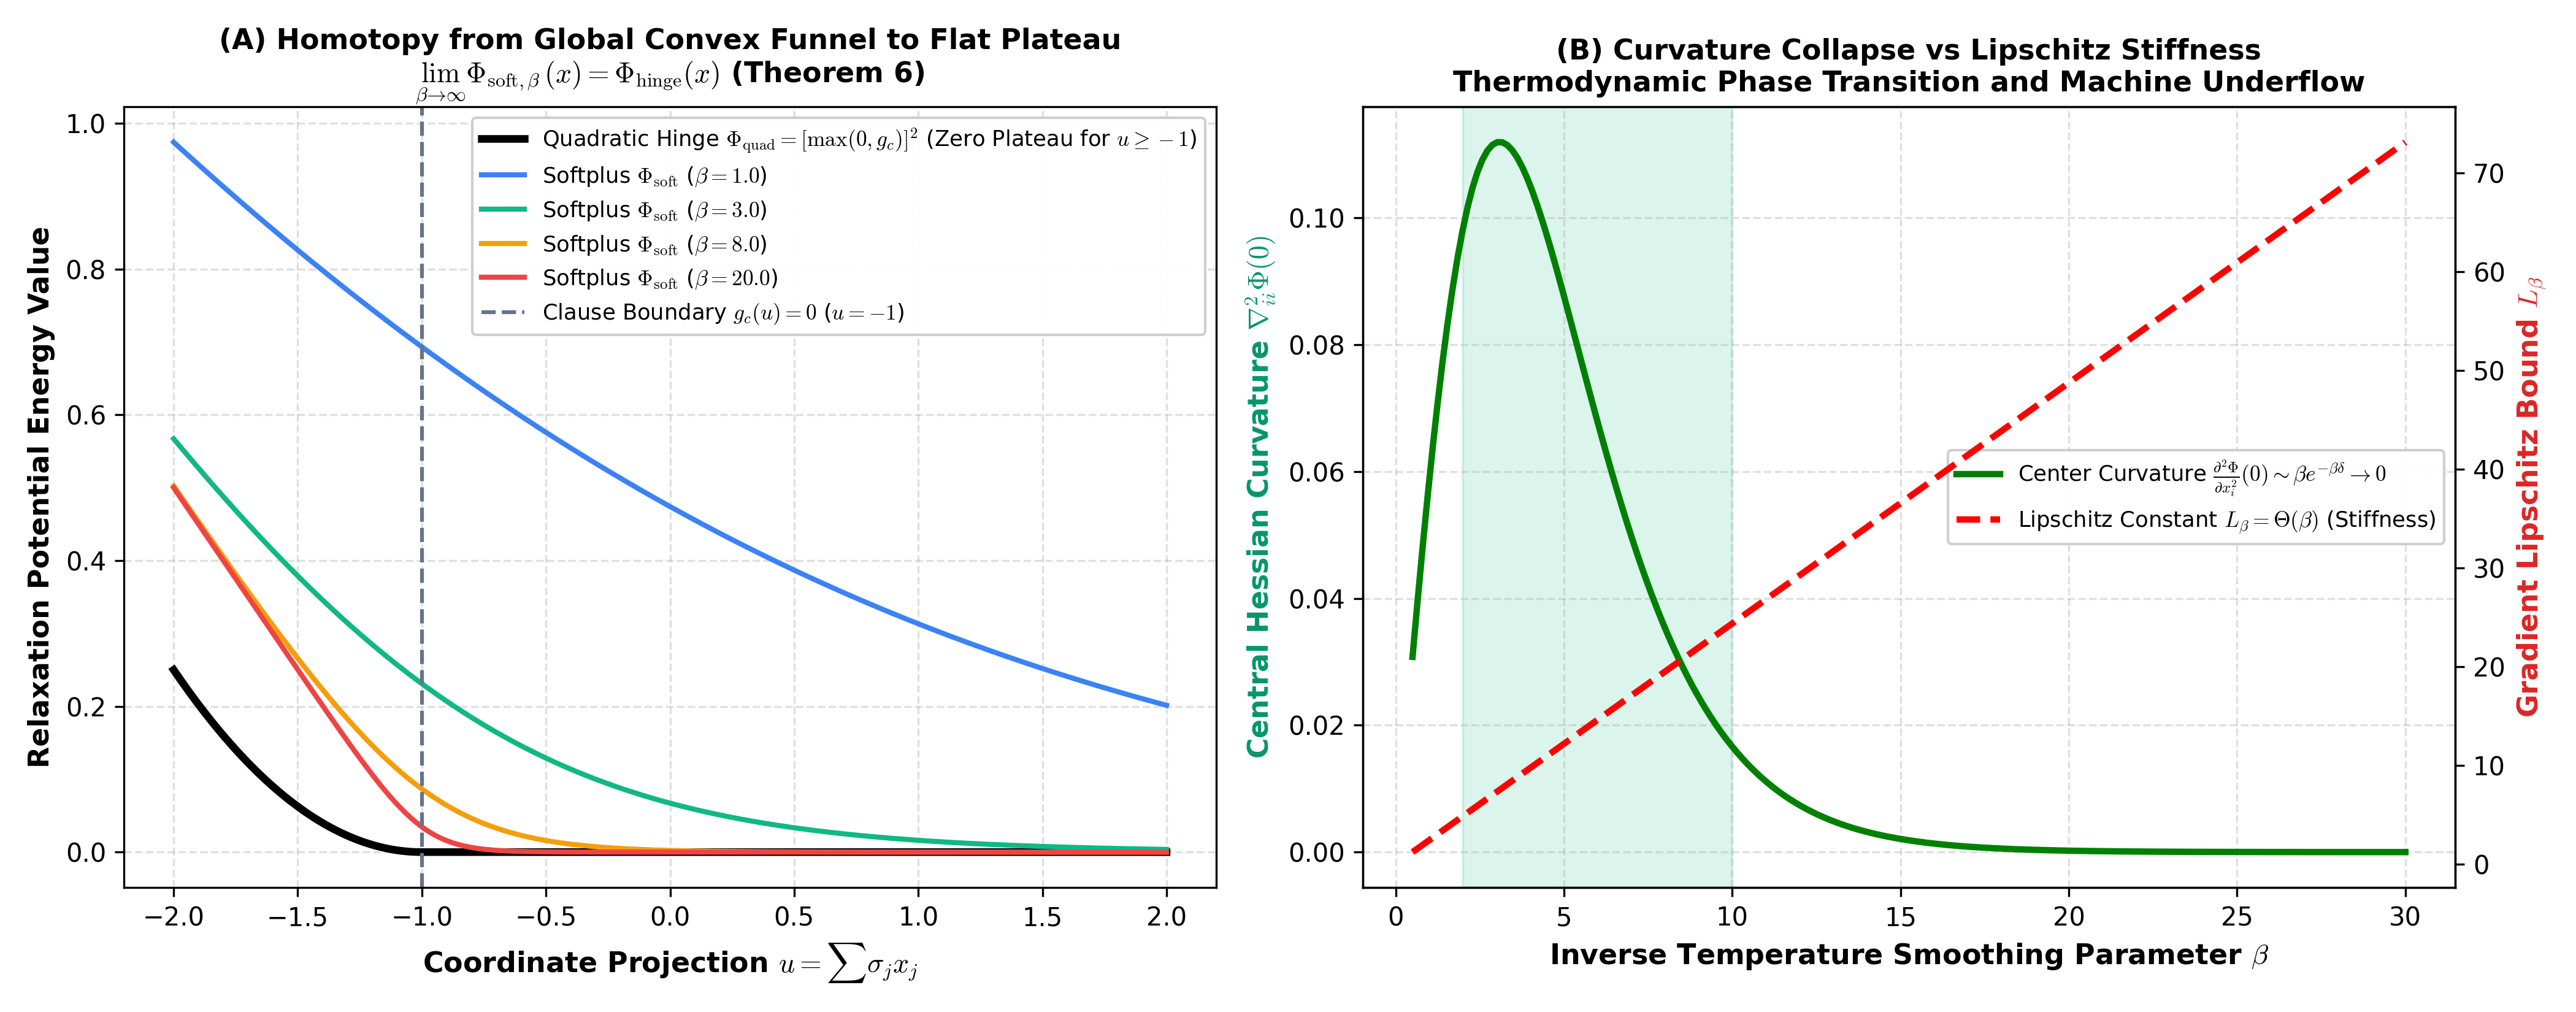
\includegraphics[width=0.80\textwidth]{../../fig_clg_teorema5_6_softplus_convexity_bifurcation.png}
\caption{Homotopia Softplus--Hinge: o aumento de $\beta$ combina rigidez global crescente com gradientes centrais exponencialmente pequenos.}
\end{figure}

\section{Contração centrípeta universal do fluxo Hinge quadrático}
Defina
\[
Z=\{x\in\mathcal X:g_c(x)\le0\ \forall c\},
\]
o politopo LP cláusula a cláusula.

\begin{theorem}[Contração centrípeta]
Para todo $x\notin Z$,
\[
\langle-\nabla\Phi_{\mathrm{quad}}(x),x\rangle
=-\sum_{c\in\operatorname{act}(x)}\bigl(2g_c(x)^2+g_c(x)\bigr)<0.
\]
Sob fluxo projetado, o raio quadrado decresce estritamente fora de $Z$. Além disso, o conjunto de equilíbrios projetados é exatamente $Z$, e toda trajetória satisfaz
\[
\operatorname{dist}(x(t),Z)\to0.
\]
\end{theorem}
\begin{proof}
Para cláusula ativa $c$, $\sigma^{(c)}\cdot x=-(2g_c+1)$ e
\[
-\nabla\Phi_{\mathrm{quad}}=\sum_{c\in\operatorname{act}}g_c\sigma^{(c)},
\]
o que fornece o produto interno acima. Escreva $v=-\nabla\Phi=d+n$ pela decomposição de Moreau, com $d=\Pi_Tv$ e $n\in N_X(x)$. Para a caixa, $\langle x,n\rangle\ge0$, de modo que $\langle x,d\rangle\le\langle x,v\rangle<0$. Isso exclui equilíbrios projetados fora de $Z$; dentro de $Z$, todos os termos Hinge estão inativos e o gradiente é nulo. O princípio de invariância de LaSalle para sistemas dinâmicos projetados fornece aproximação a $Z$ \cite{brogliato2006equivalence,nagurney1996projected}.
\end{proof}

\section{Síntese}
As três representações implementam geometrias interiores nitidamente distintas:

\begin{center}
\small
\begin{tabularx}{\textwidth}{@{}lXXX@{}}
\toprule
& Hinge & Multilinear & Softplus\\
\midrule
Massa crítica central & platô positivo & medida zero & medida zero\\
Curvatura & quadrática por partes / plana & harmônica, traço zero & $V^TWV\succeq0$\\
Mínimos interiores & pontos do platô & nenhum & único se $\operatorname{rank}(V)=N$\\
Equilíbrios projetados & exatamente o politopo LP $Z$ & conjunto de bordo dependente da representação & minimizadores do potencial convexo\\
Questão de grande parâmetro & planicidade exata & não há análogo Softplus & $L_\beta=\Theta(\beta)$ e gradiente central exponencialmente pequeno\\
\bottomrule
\end{tabularx}
\end{center}

A comparação mostra por que a concordância Booleana nos vértices é insuficiente para prever a dinâmica contínua. A representação Hinge introduz um conjunto de dimensão plena de pontos estacionários fracionários; a representação multilinear remove mínimos interiores, mas ainda pode sustentar atratores de bordo não estritos; a representação Softplus restaura convexidade ao custo de um compromisso entre rigidez e gradiente evanescente quando $\beta$ cresce.

\section{Conclusão}
Relaxações contínuas de 3-SAT que codificam as mesmas cláusulas podem possuir geometrias críticas fundamentalmente diferentes. O platô Hinge fracionário central, a extensão multilinear harmônica e a fatoração convexa Softplus definem três regimes analíticos distintos. Esses resultados determinísticos formam uma camada geométrica reutilizável para investigações probabilísticas ou algorítmicas posteriores, mas, isoladamente, não constituem afirmação sobre classes de complexidade computacional.

\begin{thebibliography}{9}
\bibitem{goemans1995improved} M. X. Goemans e D. P. Williamson, "Improved approximation algorithms for maximum cut and satisfiability problems using semidefinite programming", \emph{Journal of the ACM}, 42(6):1115--1145, 1995.
\bibitem{okamoto1973distinctness} M. Okamoto, "Distinctness of the eigenvalues of a quadratic form in a multivariate sample", \emph{Annals of Statistics}, 1(4):763--765, 1973.
\bibitem{caron2005zero} R. Caron e T. Traynor, "Zero sets of polynomials and Lebesgue measure", University of Windsor Technical Report, 2005.
\bibitem{krantz2002primer} S. G. Krantz e H. R. Parks, \emph{A Primer of Real Analytic Functions}. Birkh\"auser Boston, 2002.
\bibitem{courant1962methods} R. Courant e D. Hilbert, \emph{Methods of Mathematical Physics: Partial Differential Equations}, vol. 2. Interscience, 1962.
\bibitem{evans2010partial} L. C. Evans, \emph{Partial Differential Equations}, 2nd ed. American Mathematical Society, 2010.
\bibitem{milnor1968singular} J. Milnor, \emph{Singular Points of Complex Hypersurfaces}. Princeton University Press, 1968.
\bibitem{brogliato2006equivalence} B. Brogliato, A. Daniilidis, C. Lemar\'echal e J. Malick, "Equivalence and complementarity issues in projected dynamical systems and differential inclusions", \emph{Mathematical Programming}, 107(3):317--335, 2006.
\bibitem{nagurney1996projected} A. Nagurney e D. Zhang, \emph{Projected Dynamical Systems and Variational Inequalities with Applications}. Springer, 1996.
\end{thebibliography}
\end{document}
